%% For double-blind review submission, w/o CCS and ACM Reference (max submission space)
\documentclass[acmsmall,review,anonymous]{acmart}\settopmatter{printfolios=true,printccs=false,printacmref=false}
%% For double-blind review submission, w/ CCS and ACM Reference
%\documentclass[acmsmall,review,anonymous]{acmart}\settopmatter{printfolios=true}
%% For single-blind review submission, w/o CCS and ACM Reference (max submission space)
%\documentclass[acmsmall,review]{acmart}\settopmatter{printfolios=true,printccs=false,printacmref=false}
%% For single-blind review submission, w/ CCS and ACM Reference
%\documentclass[acmsmall,review]{acmart}\settopmatter{printfolios=true}
%% For final camera-ready submission, w/ required CCS and ACM Reference
%\documentclass[acmsmall]{acmart}\settopmatter{}


%% Journal information
%% Supplied to authors by publisher for camera-ready submission;
%% use defaults for review submission.
\acmJournal{PACMPL}
\acmVolume{1}
\acmNumber{CONF} % CONF = POPL or ICFP or OOPSLA
\acmArticle{1}
\acmYear{2018}
\acmMonth{1}
\acmDOI{} % \acmDOI{10.1145/nnnnnnn.nnnnnnn}
\startPage{1}

%% Copyright information
%% Supplied to authors (based on authors' rights management selection;
%% see authors.acm.org) by publisher for camera-ready submission;
%% use 'none' for review submission.
\setcopyright{none}
%\setcopyright{acmcopyright}
%\setcopyright{acmlicensed}
%\setcopyright{rightsretained}
%\copyrightyear{2018}           %% If different from \acmYear

%% Bibliography style
\bibliographystyle{ACM-Reference-Format}
%% Citation style
\citestyle{acmauthoryear}  %% For author/year citations
%\citestyle{acmnumeric}     %% For numeric citations
%\setcitestyle{nosort}      %% With 'acmnumeric', to disable automatic
                            %% sorting of references within a single citation;
                            %% e.g., \cite{Smith99,Carpenter05,Baker12}
                            %% rendered as [14,5,2] rather than [2,5,14].
%\setcitesyle{nocompress}   %% With 'acmnumeric', to disable automatic
                            %% compression of sequential references within a
                            %% single citation;
                            %% e.g., \cite{Baker12,Baker14,Baker16}
                            %% rendered as [2,3,4] rather than [2-4].


%%%%%%%%%%%%%%%%%%%%%%%%%%%%%%%%%%%%%%%%%%%%%%%%%%%%%%%%%%%%%%%%%%%%%%
%% Note: Authors migrating a paper from traditional SIGPLAN
%% proceedings format to PACMPL format must update the
%% '\documentclass' and topmatter commands above; see
%% 'acmart-pacmpl-template.tex'.
%%%%%%%%%%%%%%%%%%%%%%%%%%%%%%%%%%%%%%%%%%%%%%%%%%%%%%%%%%%%%%%%%%%%%%


%% Some recommended packages.
\usepackage{booktabs}   %% For formal tables:
                        %% http://ctan.org/pkg/booktabs
\usepackage{subcaption} %% For complex figures with subfigures/subcaptions
                        %% http://ctan.org/pkg/subcaption

\usepackage{tikz}
\usetikzlibrary{arrows,automata}
\usepackage{tikz-qtree} % Used for syntax trees
\usepackage{tikz-cd} % Used for commutative diagrams

\usepackage{syntax}

\usepackage{semantic}

\usepackage{marginnote}

\usepackage{listings}
\lstset{
  basicstyle=\ttfamily,
  basewidth={.5em,.5em},
}
\newcommand{\ocaml}{\lstinline[language={[objective]caml}]}

%% symbol definitions used throughout the paper

\newcommand{\NT}{\mathbb{N}} % Set of nonterminals
\newcommand{\T}{\Sigma} % Set of terminals
\newcommand{\Labels}{\mathbb{L}} % Set of labels
\newcommand{\yield}{\mathit{yield}} % yield of a parse tree
\newcommand{\semantic}{\mathit{semantic}} % remove semantically unimportant productions from a w' \in L(G')
\newcommand{\parse}{\mathit{parse}} % go from a w' \in L(G') to a subset of L(T)
\newcommand{\words}{\mathit{words}} % go from a t \in L(T) to a subset of L(G')
\newcommand{\range}[2]{#1\!-\!#2}

\begin{document}

% Submission may be up to 25 pages, excluding references

%% Title information
\title{Resolvable Ambiguity}         %% [Short Title] is optional;
                                        %% when present, will be used in
                                        %% header instead of Full Title.


%% Author information
%% Contents and number of authors suppressed with 'anonymous'.
%% Each author should be introduced by \author, followe by
%% \authornote (optional), \orcid (optional), \affiliation, and
%% \email.
%% An author may have multiple affiliations and/or emails; repeat the
%% appropriate command.
%% Many elements are not rendered, but should be provided for metadata
%% extraction tools.

%% Author with single affiliation.
\author{Viktor Palmkvist}
\authornote{with author1 note}          %% \authornote is optional;
                                        %% can be repeated if necessary
\orcid{nnnn-nnnn-nnnn-nnnn}             %% \orcid is optional
\affiliation{
  \position{Position1}
  \department{Department1}              %% \department is recommended
  \institution{KTH Royal Institute of Technology}            %% \institution is required
  \streetaddress{Street1 Address1}
  \city{Stockholm}
  \state{State1}
  \postcode{Post-Code1}
  \country{Sweden}                    %% \country is recommended
}
\email{vipa@kth.se}          %% \email is recommended

%% Author with two affiliations and emails.
\author{First2 Last2}
\authornote{with author2 note}          %% \authornote is optional;
                                        %% can be repeated if necessary
\orcid{nnnn-nnnn-nnnn-nnnn}             %% \orcid is optional
\affiliation{
  \position{Position2a}
  \department{Department2a}             %% \department is recommended
  \institution{Institution2a}           %% \institution is required
  \streetaddress{Street2a Address2a}
  \city{City2a}
  \state{State2a}
  \postcode{Post-Code2a}
  \country{Country2a}                   %% \country is recommended
}
\email{first2.last2@inst2a.com}         %% \email is recommended
\affiliation{
  \position{Position2b}
  \department{Department2b}             %% \department is recommended
  \institution{Institution2b}           %% \institution is required
  \streetaddress{Street3b Address2b}
  \city{City2b}
  \state{State2b}
  \postcode{Post-Code2b}
  \country{Country2b}                   %% \country is recommended
}
\email{first2.last2@inst2b.org}         %% \email is recommended


%% Abstract
%% Note: \begin{abstract}...\end{abstract} environment must come
%% before \maketitle command
\begin{abstract}
Text of abstract \ldots.
\end{abstract}


%% 2012 ACM Computing Classification System (CSS) concepts
%% Generate at 'http://dl.acm.org/ccs/ccs.cfm'.
\begin{CCSXML}
<ccs2012>
<concept>
<concept_id>10011007.10011006.10011008</concept_id>
<concept_desc>Software and its engineering~General programming languages</concept_desc>
<concept_significance>500</concept_significance>
</concept>
<concept>
<concept_id>10003456.10003457.10003521.10003525</concept_id>
<concept_desc>Social and professional topics~History of programming languages</concept_desc>
<concept_significance>300</concept_significance>
</concept>
</ccs2012>
\end{CCSXML}

\ccsdesc[500]{Software and its engineering~General programming languages}
\ccsdesc[300]{Social and professional topics~History of programming languages}
%% End of generated code


%% Keywords
%% comma separated list
\keywords{keyword1, keyword2, keyword3}  %% \keywords are mandatory in final camera-ready submission


%% \maketitle
%% Note: \maketitle command must come after title commands, author
%% commands, abstract environment, Computing Classification System
%% environment and commands, and keywords command.
\maketitle


\section{Introduction}

Text of paper \ldots

\subsection{Motivating Ambiguity in Programming Languages}

% TODO: reference PADL paper for this example
Consider the following nested match expression in OCaml:

\begin{lstlisting}[language={[objective]caml}]
match 1 with
  | 1 -> match "one" with
         | str -> str
  | 2 -> "two"
\end{lstlisting}

\noindent The OCaml compiler, when presented with this code, will give a type error for the last line:

\begin{lstlisting}
Error: This pattern matches values of type int
       but a pattern was expected which matches
       values of type string
\end{lstlisting}

\noindent The compiler sees the last line as belonging to the inner \ocaml{match} rather than the outer, as was intended. The fix is simple; put parentheses around the inner match:

\begin{lstlisting}[language={[objective]caml}]
match 1 with
  | 1 -> (match "one" with
          | str -> str)
  | 2 -> "two"
\end{lstlisting}

\noindent The connection between the error message and the fix is not a clear one however; adding parentheses around an expression does not change the type of anything.

To come up with an alternative error to present in this case we look to the OCaml manual for inspiration. It contains an informal description of the syntax of the language\footnote{\url{https://caml.inria.fr/pub/docs/manual-ocaml/language.html}}, in the form of an EBNF-like grammar. Below is an excerpt of the productions for expressions, written in a more standard variant of EBNF:

\setlength{\grammarindent}{5em}
\begin{grammar}
<expr> ::= 'match' <expr> 'with' <pattern-matching>

<pattern-matching> ::= ('|' <pattern> '->' <expr>)+
\end{grammar}

Note that \synt{pattern-matching} is slightly simplified, the original grammar supports \ocaml{when} guards and makes the first \lit{|} optional. If we use this grammar to parse the nested match we find an ambiguity: the last match arm can belong to either the inner match or the outer match. The OCaml compiler makes an arbitrary choice to remove the ambiguity, which may or may not be the alternative the user intended.

We instead argue that the grammar should be left ambiguous for this sort of corner cases that are likely to trip a user, allowing the compiler to present an ambiguity error, which lets the user select the intended alternative.

\subsection{Unresolvable Ambiguity}

Unfortunately, not all ambiguities can be resolved by adding parentheses. Again, looking to the informal OCaml grammar:

\setlength{\grammarindent}{5em}
\begin{grammar}
<expr> ::= <expr> ';' <expr>
  \alt '[' <expr> (';' <expr>)* ';'? ']'
  \alt <constant>
\end{grammar}

\noindent The first production is sequential composition, the second is lists (the empty list is under \synt{constant}). Now consider the following expression: ''\ocaml{[1; 2]}''.

We find that it is ambiguous with two alternatives:
\begin{enumerate}
  \item A list with two elements.
  \item A list with one element, namely a sequential composition.
\end{enumerate}

We can select the second option by putting parentheses around ''\ocaml{1; 2}'', but there is no way to select the first. If the user intended the first option we have a problem: we can present an accurate error message, but there is no way for an end-user to solve it; it requires changes to the grammar itself.

To prevent the possibility of an end-user encountering such an error we must ensure that the grammar cannot give rise to an unresolvable ambiguity. It is worth mentioning here that statically checking if a context-free grammar is ambiguous has long been known to be undecidable \cite{cantorAmbiguityProblemBackus1962}. Unresolvable ambiguity, however, turns out to be decidable\footnote{With some caveats, I'll talk more about this during the meeting.}.

Note that, as for ambiguity, the shape of the grammar is important, since the property considers parse trees rather than merely words. For this paper, we consider context-free grammars with EBNF operators.

\subsection{Contributions}

\begin{itemize}
  \item Building on the work by \citet{palmkvistCreatingDomainSpecificLanguages2019}, which merely isolates ambiguities, an algorithm that suggests solutions to ambiguity errors.
  \item A formalization of the unresolvable ambiguity property for context-free EBNF grammars.
  \item An algorithm for deciding if a grammar is unresolvably ambiguous or not.
\end{itemize}

\section{Preliminaries}

\begin{quote} % TODO: remove
  \textbf{NOTE:} The text before this section is largely out of date.
\end{quote}
% TODO: note that the syntax tree definition is a little bit non-standard

\subsection{Context-Free Grammars}

A context-free grammar $G$ is a tuple $(\NT, \T, P, S)$ where:

\begin{itemize}
\item $\NT$ is a set of non-terminals.
\item $\T$, disjoint from $\NT$, is a set of terminals.
\item $P$, a subset of $\NT \times (\NT \cup \T)^{*}$, is a set of productions.
\item $S \in \NT$ is the starting non-terminal.
\end{itemize}

\noindent A word $w \in \T^{*}$ is recognized by $G$ if there is a sequence of steps starting with $S$ and ending with $w$, where each step replaces a single non-terminal using a production in $P$. The set of words recognized by $G$ is written $L(G)$, and is said to be the word language of $G$.

\subsection{Syntax Trees}

A syntax tree takes the terminals of a word and arranges them into a tree, the shape of which is determined by how (i.e., using which productions) the word was parsed / recognized. For this paper we will use a linear encoding of syntax trees, letting us use context-free grammars to express the set of syntax trees for some given word language. For example, the parse trees of a context-free grammar $G_w = (\NT, \T, P, S)$ are described by the context-free grammar $G_t = (\NT, \T \cup \T_{[]}, P', S)$ where:

\begin{itemize}
\item $T_{[]} = \bigcup_{p \in P} \{ [_p, ]_p \}$, i.e., a unique pair of brackets per production.
\item $P' = \{ N -> [_p \alpha ]_p \mid p \in P \land p = N -> \alpha \}$, i.e., each production is wrapped with a unique pair of brackets.
\end{itemize}

\noindent Such a grammar will (slightly erroneously) be referred to as a tree grammar, and the recognized language as a tree language. We will also use syntax trees that are not directly derived from the parse trees of a context-free grammar. The precise construction of these will be described at the point of their introduction, but the basic process is the same; surround each production with a unique pair of brackets.

% TODO: reference a book on tree automata and languages
As such we can define a function $\yield$ (as seen, e.g., in ) that takes a tree and flattens it, producing the word it was constructed from. Intuitively, this function merely removes the added brackets.

\subsection{Ambiguity}

The standard definition of ambiguity, using the above formulation of syntax trees, is as follows:

\begin{definition}
A word $w \in L(G_w)$ is ambiguous relative its parse tree $G_t$ if:
  \[ \exists t_1, t_2 \in L(G_t).\ t_1 \neq t_2 \land \yield(t_1) = w = \yield(t_2)\]
\end{definition}

\noindent For this paper, we widen the definition slightly to the following:

\begin{definition}
  A word $w \in L(G_w)$ is ambiguous relative a tree grammar $G_t$ and a function $\parse : L(G_w) -> 2^{L(G_t)}$ if:
  \[ |\parse(w)| > 1 \]
\end{definition}

\noindent where $2^S$ is the powerset of $S$ and $|S|$ is the cardinality of $S$. The standard ambiguity definition is regained by choosing

\[ \parse(w) = \{ t \mid w = \yield(t) \land t \in L(G_t) \}\ \]

\subsection{Automata}

A nondeterministic finite automaton (NFA) is a tuple $(Q, \Sigma, \delta, q_0, F)$:

\begin{itemize}
\item A finite set of states $Q$.
\item A finite set of input symbols $\Sigma$, i.e., an input alphabet.
\item A transition function $\delta: Q \times \Sigma -> 2^Q$.
\item An initial state $q_0 \in Q$.
\item A set of final states $F \subseteq Q$.
\end{itemize}

\noindent A successful run is a sequence of states $r_0, r_1, \ldots, r_n$ and a word $a_0a_1\ldots a_n$ such that:

\begin{itemize}
\item $r_0 = q_0$.
\item $\forall i \in \{0, 1, \ldots, n-1\}.\ r_{i+1} \in \delta(r_i, a_i)$.
\item $r_n \in F$.
\end{itemize}

\noindent We say that the automaton accepts the word $a_0a_1\ldots a_n$ iff there is such a succesful run.

A deterministic finite automaton (DFA) has the same definition, except $\delta : Q \times \Sigma -> Q$, i.e., given a state and a symbol there is always a single state we can transition to.

A pushdown automaton extends a finite automaton with a stack, and lets each transition push or pop symbols from it. Formally, a nondeterministic pushdown automaton is a tuple $(Q, \Sigma, \Gamma, \delta, q_0, F)$:

\begin{itemize}
\item A finite set of states $Q$.
\item A finite set of input symbols $\Sigma$, i.e., an input alphabet.
\item A finite set of stack symbols $\Gamma$, i.e., a stack alphabet.
\item A transition function $\delta: Q \times \Sigma \times \Gamma -> 2^{Q \times \Gamma^{*}}$.
\item An initial state $q_0 \in Q$.
\item A set of final states $F \subseteq Q$.
\end{itemize}

\noindent A successful run is now a sequence of \emph{configurations}, elements of $Q \times \Gamma^{*}$, starting with $(q_0, \epsilon)$, ending with $(f, \gamma)$ for some $f \in F$ and $\gamma \in \Gamma*$.

However, in this paper we will only consider pushdown automata with relatively limited stack manipulation, and will thus use some convenient shorthand:

\begin{itemize}
\item $p \xrightarrow{a} q$, a transition that recognizes the terminal $a$ and does not interact with the stack at all.
\item $p \xrightarrow{a, +g} q$, a transition that recognizes the terminal $a$ and pushes the symbol $g$ on the stack.
\item $p \xrightarrow{a, -g} q$, a transition that recognizes the terminal $a$ and pops the symbol $g$ from the stack (i.e., this transition cannot be taken if $g$ is not on top of the stack).
\end{itemize}

\subsection{Visibly Pushdown Languages}

A visibly pushdown language \cite{alurVisiblyPushdownLanguages2004} is a language that can be recognized by a visibly pushdown automaton. A visibly pushdown automaton is a pushdown automaton where the input alphabet $\Sigma$ can be partitioned into three disjoint sets $\Sigma_c$, $\Sigma_i$, and $\Sigma_r$, such that all transitions in the automaton has one of the following three forms:

\begin{itemize}
\item $p \xrightarrow{c, +s} q$, where $c \in \Sigma_c$.
\item $p \xrightarrow{i} q$, where $i \in \Sigma_i$.
\item $p \xrightarrow{r, -s} q$, where $r \in \Sigma_r$.
\end{itemize}

\noindent i.e., the terminal recognized by a transition fully determines the change to the stack height.

This gives us some nice properties. Of particular relevance to this paper are the following two points:

\begin{itemize}
\item If two visibly pushdown automata have the same partitions $\Sigma_c$, $\Sigma_i$, and $\Sigma_r$, then we can construct a product automaton that simulates two simultaneous runs through both automata. This product automaton has the same input alphabet partitions, each state is a pair of states (one from each automaton), and each stack symbol is a pair of stack symbols (one from each automaton).
\item A visibly pushdown automaton can be trimmed \cite{caralpTrimmingVisiblyPushdown2013}, i.e., modified in such a way that all remaining states and transitions are part of at least one successful run, none are redundant.
\end{itemize}

\section{Parse-time Disambiguation}

We begin this section with some motivation, then list our definition of \emph{resolvable ambiguity} and what disambiguation we will consider, and finally an alternative definition of a word, which will be useful in later sections.

We can divide the productions present in a programming language grammar in two groups: those that are semantically important, and those that are semantically \emph{un}important. The former group covers most productions, while the latter contains, e.g., parentheses used for explicit grouping. If programs were written directly as syntax trees then the latter would be unnecessary; two syntax trees that differ only by parentheses are semantically the same.

Thus we wish the output of parsing to be a syntax tree consisting entirely of semantically important productions. This distinction is useful to make, because it allows us to decouple \emph{what} we want to be expressible and \emph{how} it is to be expressed.

\begin{figure}
  \begin{tabular}{@{}ll@{}}
      Terminals & $t \in \T$ \\
      Non-terminals & $N \in \NT$ \\
      Labels & $l \in \Labels$ \\
      Marks & $m \subseteq \Labels$ \\
      Regular expressions & $r ::= t \mid N_m \mid r \cdot r \mid r + r \mid \epsilon \mid r^{*}$ \\
      Labelled productions & $N -> l : r$ \\
  \end{tabular}
  \caption{The abstract syntax of a language definition.}
  \label{fig:input-language-definition}
\end{figure}

\begin{figure}
  \begin{tabular}{@{}l@{\quad$->$\quad}l@{ $:$\quad}l@{}}
    $E$ & $l$ & \verb|'['| ($E$ (\verb|';'| $E$)$^{*}$ $+$ $\epsilon$) \verb|']'| \\
    $E$ & $a$ & $E$ \verb|'+'| $E$ \\
    $E$ & $m$ & $E_{\{a\}}$ \verb|'*'| $E_{\{a\}}$ \\
    $E$ & $n$ & $N$ \\
  \end{tabular}
  \caption{The input language definition used as a running example, an expression language with lists, addition, and multiplication, with precedence defined, but not associativity. Assumes that $N$ matches a numeric terminal.}
  \label{fig:running-example-definition}
\end{figure}

With that in mind, we define a language definition $D$ as a set of labelled productions, as described in Figure~\ref{fig:input-language-definition}. Note that we require the labels to uniquely identify the production, i.e., there can be no two distinct productions in $D$ that share the same label. A \emph{mark} is used for disambiguation, and forbids certain productions from taking the place of the marked non-terminal. To lessen clutter, we will write $E_\emptyset$ as $E$. As an example, consider the language definition in Figure~\ref{fig:running-example-definition}, which will be used as a running example. In the production describing multiplication ($m$) both non-terminals are marked with $\{a\}$, which thus forbids addition from being a child of a multiplication, enforcing conventional precedence.

From $D$ we then generate four grammars: $G_w$, $G_t$, $G'_w$, and $G'_t$. The first two represent the \emph{what}, while the latter two represent the \emph{how}:

\begin{itemize}
\item $G_w$ represents a word language describing all semantically distinct programs.
\item $G_t$ represents a tree language describing the syntax trees obtained by parsing a word in $L(G_w)$. Note that the added brackets are not present in the productions of $E_{l1}$ and $E_{l2}$, since those are all part of the same labelled production in $D$ in Figure~\ref{fig:running-example-definition}.
\item $G'_w$ is essentially a modified version of $G_w$, e.g., adding parentheses and other forms of disambiguation.
\item $G'_t$ represents a tree language describing the syntax trees obtained by parsing a word in $L(G'_w)$.
\end{itemize}

\begin{figure}
  \begin{subfigure}[t]{.45\linewidth}
    \centering
    \begin{tabular}{@{}l@{\quad$->$\quad}l@{}}
      \toprule
      $E$ & \verb|'['| $E_{l1}$ \verb|']'| \\
      $E$ & $E$ \verb|'+'| $E$ \\
      $E$ & $E$ \verb|'*'| $E$ \\
      $E$ & $N$ \\
      \midrule
      $E_{l1}$ & $\epsilon$ \\
      $E_{l1}$ & $E$ $E_{l2}$ \\
      \midrule
      $E_{l2}$ & $\epsilon$ \\
      $E_{l2}$ & \verb|';'| $E$ $E_{l2}$ \\
      \bottomrule
    \end{tabular}
    \caption{$G_w$, the generated abstract syntax.}
    \label{fig:running-example-generated:w}
  \end{subfigure}%
%
  \begin{subfigure}[t]{.54\linewidth}
    \centering
    \begin{tabular}{@{}l@{\quad$->$\quad}lll@{}}
      \toprule
      $E$ & $[_{l}$ & \verb|'['| $E_{l1}$ \verb|']'| & $]_{l}$ \\
      $E$ & $[_{a}$ & $E$ \verb|'+'| $E$ & $]_{a}$ \\
      $E$ & $[_{m}$ & $E$ \verb|'*'| $E$ & $]_{m}$ \\
      $E$ & $[_{n}$ & $N$ & $]_{n}$ \\
      \midrule
      $E_{l1}$ & & $\epsilon$ & \\
      $E_{l1}$ & & $E$ $E_{l2}$ & \\
      \midrule
      $E_{l2}$ & & $\epsilon$ & \\
      $E_{l2}$ & & \verb|';'| $E$ $E_{l2}$ & \\
      \bottomrule
    \end{tabular}
    \caption{$G_t$, a language describing a linear encoding of the parse trees of $G_w$.}
    \label{fig:running-example-generated:t}
  \end{subfigure}

  \begin{subfigure}[t]{.45\linewidth}
    \centering
    \begin{tabular}{@{}l@{\quad$->$\quad}l@{}}
      \toprule
      $E$ & \verb|'['| $E_{l1}$ \verb|']'| \\
      $E$ & $E$ \verb|'+'| $E$ \\
      $E$ & $E_{\{a\}}$ \verb|'*'| $E_{\{a\}}$ \\
      $E$ & $N$ \\
      $E$ & \verb|'('| $E$ \verb|')'| \\
      \midrule
      $E_{\{a\}}$ & \verb|'['| $E_{l1}$ \verb|']'| \\
      $E_{\{a\}}$ & $E_{\{a\}}$ \verb|'*'| $E_{\{a\}}$ \\
      $E_{\{a\}}$ & $N$ \\
      $E_{\{a\}}$ & \verb|'('| $E$ \verb|')'| \\
      \midrule
      $E_{l1}$ & $\epsilon$ \\
      $E_{l1}$ & $E$ $E_{l2}$ \\
      \midrule
      $E_{l2}$ & $\epsilon$ \\
      $E_{l2}$ & \verb|';'| $E$ $E_{l2}$ \\
      \bottomrule
    \end{tabular}
    \caption{$G'_w$, the generated concrete syntax.}
    \label{fig:running-example-generated:w-prime}
  \end{subfigure}%
%
  \begin{subfigure}[t]{.54\linewidth}
    \centering
    \begin{tabular}{@{}l@{\quad$->$\quad}lll@{}}
      \toprule
      $E$ & $[_{l, \emptyset}$ & \verb|'['| $E_{l1}$ \verb|']'| & $]_{l, \emptyset}$ \\
      $E$ & $[_{a, \emptyset}$ & $E$ \verb|'+'| $E$ & $]_{a, \emptyset}$ \\
      $E$ & $[_{m, \emptyset}$ & $E_{\{a\}}$ \verb|'*'| $E_{\{a\}}$ & $]_{m, \emptyset}$ \\
      $E$ & $[_{n, \emptyset}$ & $N$ & $]_{n, \emptyset}$ \\
      $E$ & $[_{g, \emptyset}$ & \verb|'('| $E$ \verb|')'| & $]_{g, \emptyset}$ \\
      \midrule
      $E_{\{a\}}$ & $[_{l, \{a\}}$ & \verb|'['| $E_{l1}$ \verb|']'| & $]_{l, \{a\}}$ \\
      $E_{\{a\}}$ & $[_{m, \{a\}}$ & $E_{\{a\}}$ \verb|'*'| $E_{\{a\}}$ & $]_{m, \{a\}}$ \\
      $E_{\{a\}}$ & $[_{n, \{a\}}$ & $N$ & $]_{n, \{a\}}$ \\
      $E_{\{a\}}$ & $[_{g, \{a\}}$ & \verb|'('| $E$ \verb|')'| & $]_{g, \{a\}}$ \\
      \midrule
      $E_{l1}$ & & $\epsilon$ & \\
      $E_{l1}$ & & $E$ $E_{l2}$ & \\
      \midrule
      $E_{l2}$ & & $\epsilon$ & \\
      $E_{l2}$ & & \verb|';'| $E$ $E_{l2}$ & \\
      \bottomrule
    \end{tabular}
    \caption{$G'_t$, a language describing a linear encoding of the parse trees of $G'_w$.}
    \label{fig:running-example-generated:t-prime}
  \end{subfigure}%
  \caption{The generated grammars.}
  \label{fig:running-example-generated}
\end{figure}

\noindent Examples of words in each of these four languages can be seen in Figure~\ref{fig:example-words-in-square}, along with visualizations of the syntax trees.

{
\newcommand{\terminal}[1]{\ \underline{#1}\ }

\begin{figure}
  \begin{subfigure}[b]{.40\linewidth}
    \[1 + 2 * 3\]
    \caption{Example word in $L(G_w)$.}
  \end{subfigure}
  \begin{subfigure}[b]{.55\linewidth}
    \begin{center}
    \Tree [.{$m$}
        [.{$a$}
          [.{$n$} 1 ]
          +
          [.{$n$} 2 ] ]
        *
        [.{$n$} 3 ] ]
    \end{center}
    \[[_m [_a [_n \terminal{1} ]_n \terminal{+} [_n \terminal{2} ]_n ]_a \terminal{*} [_n \terminal{3} ]_n ]_m\]
    \caption{Example word in $L(G_T)$ and visualized tree.}
  \end{subfigure}

  \begin{subfigure}[b]{.40\linewidth}
    \[(1 + 2) * 3\]
    \caption{Example word in $L(G'_w)$.}
  \end{subfigure}
  \begin{subfigure}[b]{.55\linewidth}
    \begin{center}
    \Tree [.{$m, \emptyset$}
        [.{$g, \{a\}$}
          (
          [.{$a, \emptyset$}
            [.{$n, \emptyset$} 1 ]
            +
            [.{$n, \emptyset$} 2 ] ]
          ) ]
        *
        [.{$n, \{a\}$} 3 ] ]
    \end{center}
    \[[_{m} [_{g, \{a\}} \terminal{(} [_{a} [_{n} \terminal{1} ]_{n} \terminal{+} [_{n} \terminal{2} ]_{n} ]_{a} \terminal{)} ]_{g, \{a\}} \terminal{*} [_{n, \{a\}} \terminal{3} ]_{n, \{a\}} ]_{m}\]
    \caption{Example word in $L(G'_T)$ and visualized tree.}
  \end{subfigure}
  \caption{Example with words from each grammar that correspond to each other. We abbreviate $[_{n, \emptyset}$ as $[_n$. The non-bracket terminals in the tree languages appear underlined for increased clarity.}
  \label{fig:example-words-in-square}
\end{figure}
}

At this point we also note that the shape of $D$ determines where the final concrete syntax permits grouping parentheses. For example, $G_w$ in Figure~\ref{fig:running-example-generated:w} can be seen as a valid language definition (if we generate new unique labels for each of the productions). However, starting with that language definition would allow the expression ''$[1(;2)]$'', which makes no intuitive sense; grouping parentheses should only be allowed around complete expressions, but ''$;2$'' is not a valid expression.

As an example, in Figure~\ref{fig:example-grammar}, \ref{fig:example-grammar:ambig-grammar} is the \emph{what} and \ref{fig:example-grammar:unambig-grammar} is the \emph{how}. The latter grammar is a modification of the former that adds precedence, associativity, and parentheses, yielding an unambiguous grammar with at least one way to express each semantically distinct tree.

\begin{figure*}
  \begin{subfigure}{.45\linewidth}
    \setlength{\grammarindent}{5em}
    \begin{grammar}
      <expr> ::= Sum: <expr> '+' <expr>
        \alt Product: <expr> '*' <expr>
        \alt Number: <number>
    \end{grammar}
    \caption{The (ambiguous) intuitive grammar without parentheses.}
    \label{fig:example-grammar:ambig-grammar}
  \end{subfigure}
  \begin{subfigure}{0.45\linewidth}
    \setlength{\grammarindent}{5em}
    \begin{grammar}
      <expr> ::= Sum: <product> '+' <expr>
        \alt PassthroughE: <product>

      <product> ::= Product: <atom> '*' <product>
        \alt PassthroughP: <atom>

      <atom> ::= Paren: '(' <expr> ')'
        \alt Number: <number>
    \end{grammar}
    \caption{The (unambiguous) grammar with parentheses.}
    \label{fig:example-grammar:unambig-grammar}
  \end{subfigure}

  \begin{subfigure}{.55\linewidth}
    \begin{center}
    \Tree [.PassthroughE
      [.\underline{Product}
        [.Paren
          '('
          [.\underline{Sum}
            [.PassthroughP [.\underline{Number} 1 ] ]
            '+'
            [.PassthroughE [.PassthroughP [.\underline{Number} 2 ] ] ] ]
          ')' ]
        '*'
        [.PassthroughP [.\underline{Number} 3 ] ] ] ]
    \end{center}
    \caption{Parse tree for $(1 + 2) * 3$. The underlined nodes are semantically important.}
    \label{fig:example-grammar:tree}
  \end{subfigure}
  \begin{subfigure}{.35\linewidth}
    \begin{center}
    \Tree [.\underline{Product}
      [.\underline{Sum} [.\underline{Number} 1 ] '+' [.\underline{Number} 2 ] ]
      '*'
      [.\underline{Number} 3 ] ]
    \end{center}
    \caption{The same parse tree, after removing the semantically unimportant nodes.}
    \label{fig:example-grammar:sem-tree}
  \end{subfigure}

  \caption{A basic expression grammar in two variations, and two example syntax trees.}
  \label{fig:example-grammar}
\end{figure*}

Our definition thus refers to four grammars in total:

\begin{itemize}
  \item The semantic grammar $G$, containing only the semantically important productions (e.g., Figure~\ref{fig:example-grammar:ambig-grammar}).
  \item $T_G$ (generally abbreviated as $T$), the parse trees of $G$, representing the trees that must be expressible (Figure~\ref{fig:example-grammar:sem-tree} is in this language).
  \item The parse grammar $G'$, a modification of $G$ meant to actually be used for parsing (e.g., Figure~\ref{fig:example-grammar:unambig-grammar}). The identifiers in this grammar need not be unique, but should be a superset of the identifiers in $G$. The modifications we will consider in this paper are introduced in Section~\ref{sec:modifications}.
  \item $T_{G'}$ (generally abbreviated as $T'$), the parse trees of $G'$ (Figure~\ref{fig:example-grammar:tree} is in this language).
\end{itemize}

\noindent We also require a function $\semantic : L(T') -> L(T)$ that removes the semantically unimportant productions from a parse tree. The relation between the four grammars can be seen in Figure~\ref{fig:grammar-square}. Finally, we define the function $\parse : L(G') -> 2^{L(T)}$, and its inverse $\words : L(T) -> 2^{L(G')}$:

$$
\begin{array}{rcl}
\parse(w') & = & \{ \semantic(t') \mid t' \in L(T') \land \yield(t') = w' \} \\
\words(t) & = & \{ w' \mid t \in \parse(w') \} \\
\end{array}
$$

\noindent The latter will be useful later, while $\parse$ is used directly in the definition of resolvable ambiguity:

\begin{figure}
  \begin{tikzcd}
    L(G) & L(T) \arrow[l, "\yield"] \\
    L(G') & L(T') \arrow[u, "\semantic"'] \arrow[l, "\yield"]
  \end{tikzcd}
  \caption{The grammars considered, and their relation to each other. $G$ is provided by a user of the system, along with instructions how to modify $G$ to construct $G'$, while $T$ and $T'$ are automatically derived.}
  \label{fig:grammar-square}
\end{figure}

\begin{definition}
  A language defined by the semantic grammar $G$ and the parse grammar $G'$ is resolvable if:
  $$
  \begin{array}{l}
  \forall t \in L(T_G).\\
  \quad \exists w' \in L(G').\ \parse(w') = \{t\}
  \end{array}
  $$
\end{definition}

\noindent Intuitively, a language is resolvably ambiguous if there is at least one (unambiguous\footnote{For a slightly different meaning of unambiguous, it's here relating $G'$ to $T$, instead of $G'$ to $T'$.}) word for each semantically distinct tree. Note that neither $G$ nor $G'$ necessarily need to be unambiguous for this to hold.

\subsection{Modifications in G'} \label{sec:modifications} % TODO: can't typeset G' in mathmode for some reason

For this paper we consider two possible modifications:

\begin{itemize}
\item Adding parentheses for explicit grouping.
\item Forbidding non-terminals in certain positions from expanding using certain productions.
\end{itemize}

\noindent The latter requires more explanation. As an example, in the following grammar we are forbidding the second \synt{<expr>} in the first production from expanding using the ''Sum'' production:

\setlength{\grammarindent}{5em}
\begin{grammar}
  <expr> ::= Sum: <expr> '+' <expr>$_{Sum}$
    \alt Number: <number>
\end{grammar}

\noindent Transforming this into a normal grammar, and adding parentheses, we get the following:

\setlength{\grammarindent}{6em}
\begin{grammar}
  <expr> ::= Sum: <expr> '+' <expr>$_{Sum}$
  \alt Number: <number>
  \alt Paren: '(' <expr> ')'

  <expr$_{Sum}$> ::= Number: <number>
  \alt Paren: '(' <expr> ')'
\end{grammar}

\noindent In other words, we produce a grammar where addition is left-associative\footnote{I'm having some issues typesetting this appropriately, and I'm not all that happy with the explanation.}, but we can use explicit grouping via parentheses to override that.

\subsection{An Alternative Word View} \label{sec:word-view}

This section introduces an alternative (isomorphic) definition of a word that will be used to motivate the correctness of later algorithms. The method by which we generate $G_w$ and $G'_w$ limits the possible differences between them significantly. In particular, no new terminals are introduced, except '(' and ')', and they are always introduced in a well-balanced fashion.

If we thus delimit ourselves to only consider languages where words have no unbalanced parentheses\footnote{I.e., the vast, vast majority of programming languages currently in use.} we can give the following alternative definition of a word: a word is a two-tuple containing a sequence of non-parenthesis terminals and a bag (or multiset) of ranges covered by parentheses. For example, the word ''$(1 + 2) * 3$'' is equivalent to $(\text{''}1 + 2 * 3\text{''}, \{\range{1}{3}\})$, while ''$((1 + 2)) * 3$'' is equivalent to $(\text{''}1 + 2 * 3\text{''}, \{\range{1}{3}, \range{1}{3}\})$. The first component will be referred to as a \emph{basic word}, the second as a \emph{range bag}

We will now note a few things about the words $w' \in \words(t)$ for some given $t \in L(G_t)$:

\begin{itemize}
\item All $w'$ have the same basic word. $G'_w$ is constructed in such a way that the only possible difference is one of parentheses. This also implies that two trees that share a word (i.e., that can be ambiguous) must also share a basic word.
\item Some parentheses are required, i.e., some ranges must be present in all $w'$. For example, removing the parentheses in ''$(1 + 2) * 3$'' changes the tree produced, since multiplication has higher precedence than addition.
\item There is a finite set of possible ranges in the range bags of $w'$. Grouping parentheses can only be added if they exactly cover a node in the parse tree, and other parentheses can only be added where $G_w$ allows them.
\item Duplicated grouping parentheses do not matter. For example, $((1 + 2)) * 3$ permits the same syntax trees as $(1 + 2) * 3$. If there are no parentheses present in $G_w$ then all parentheses are grouping parentheses, thus we can consider the range bag as a \emph{set} instead.
\end{itemize}

\section{Static Resolvability Check}

This section describes a decision algorithm for detecting unresolvable ambiguities in a language definition, starting with a version with several limitations, most of which are later lifted. The overarching goal is to find a tree $t \in L(G_t)$ such that there is no $w' \in L(G'_w)$ for which $\parse(w') = \{t\}$. Alternatively, find a tree that has no unambiguous words.

\subsection{Basic Algorithm}

Our initial limitations / assumptions are as follows:

\begin{enumerate}
  \item The input language definition contains no parentheses. This implies that all parentheses in $G'_w$ are grouping parentheses, thus we only need to consider words $w' \in L(G'_w)$ whose range bag is a set.

  \item No non-terminals in the input language definition are marked, i.e., there are no forbidden children. This implies that there are no required grouping parentheses.

  \item No production has a right-hand side that matches a single non-terminal, i.e., $\forall (N->i:r) \in D.\ \NT \cap L(r) = \emptyset$\footnote{I haven't really written a proper description for the language definition, but I'm here using $D$ for it, and considering it essentially as a set of ''productions''.}.
\end{enumerate}

\noindent The first two limitations allow us to place all words in $\words(t)$ for some given $t$ in a lattice, whose structure is formed by the subset ordering of the range sets. For example, the two trees in Figure~\ref{fig:ambig-example-square} have the lattices of words seen in Figures~\ref{fig:lattice1} and \ref{fig:lattice2} respectively.

The bottom word corresponds to the set of required parentheses (i.e., the empty set, in this sub-problem), while the top word corresponds to the set of possible parentheses ranges. All trees that can be ambiguous must thus share the same bottom word, while the top may differ.

Of particular use is to examine whether the top word (call it $w'$) is ambiguous. There are two cases:

\begin{itemize}
\item The top word is unambiguous, then this is not a tree we are looking for (since it has at least one unambiguous word).
\item It is ambiguous. That means that there is some other lattice for some other tree that also contains the word. Call the top word of this other lattice $w'_2$. For $w'$ to be in the lattice whose top is $w'_2$ its rangeset must be a subset of the rangeset of the latter. But this is true also for all the other words in the lattice, thus there are no unambiguous words in the lattice, i.e., this tree is what we are looking for.
\end{itemize}

\noindent The algorithm thus looks for two trees, where the set of possible parentheses for one is a superset of the other. To do this, we use a linear representation of each lattice: namely the top word. If two trees have the same top word, that implies that their sets of possible parentheses are equal. If we can add parentheses to one word and get the other word, that implies that the rangeset of the former is a subset of the latter.

We will now construct a pushdown automaton that recognizes these top words in such a way that there is a bijection between successful runs and trees in $L(G_t)$. As a running example, we will use the following (very simple) language definition $D$:

\begin{center}
\begin{tabular}{@{}l@{\quad$->$\quad}l@{ $:$\quad}l@{}}
  \synt{N} & Succ & 's' \synt{N}\\
  \synt{N} & Zero & 'z' \\
\end{tabular}
\end{center}

\noindent We begin by constructing a DFA per production. This can be done in the standard way by constructing an NFA, then determinizing it, and optionally minimizing it.

\begin{center}
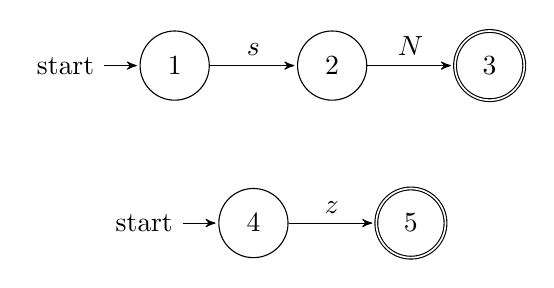
\begin{tikzpicture}[->,>=stealth',shorten >=1pt,auto,node distance=2cm,
    scale = 1,transform shape]

  \node[state,initial] (1) {$1$};
  \node[state] (2) [right of=1] {$2$};
  \node[state,accepting] (3) [right of=2] {$3$};
  \node[state,initial] (4) [below of=1, xshift=1cm] {$4$};
  \node[state,accepting] (5) [right of=4] {$5$};

  \path (1) edge              node {$s$} (2)
  (2) edge              node {$N$} (3)
  (4) edge              node {$z$} (5);

\end{tikzpicture}
\end{center}

\noindent We then combine them into a single pushdown automata by replacing each edge with a non-terminal label $p \xrightarrow{N} q$ with:

\begin{itemize}
  \item an edge $p \xrightarrow{'(', +(p, q)} p'$ for every initial state $p'$ in some DFA belonging to non-terminal $N$, and
  \item an edge $q' \xrightarrow{')', -(p, q)} q$ for every final state $q'$ in some DFA belonging to non-terminal $N$,
\end{itemize}

\noindent Intuitively, we parse a child node, but put parentheses around it, then return. This is where we use assumption 3, without it we might introduce double parentheses here.

\begin{center}
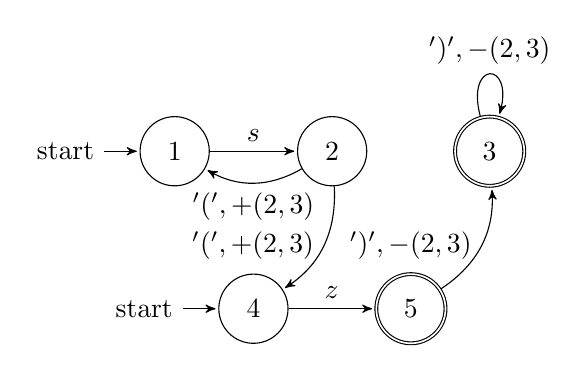
\begin{tikzpicture}[->,>=stealth',shorten >=1pt,auto,node distance=2cm,
    scale = 1,transform shape]

  \node[state,initial] (1) {$1$};
  \node[state] (2) [right of=1] {$2$};
  \node[state,accepting] (3) [right of=2] {$3$};
  \node[state,initial] (4) [below of=1, xshift=1cm] {$4$};
  \node[state,accepting] (5) [right of=4] {$5$};

  \draw
  (1) edge[above] node{$s$} (2)
  (4) edge[above] node{$z$} (5)
  (2) edge[bend left, below] node{$'(', +(2, 3)$} (1)
  (2) edge[bend left, left] node{$'(', +(2, 3)$} (4)
  (3) edge[loop above] node{$')', -(2, 3)$} (3)
  (5) edge[left, bend right] node{$')', -(2, 3)$} (3);

\end{tikzpicture}
\end{center}

\noindent Finally, we add a new initial state and a new final state, and connect them with the initial and final states belonging to the starting non-terminal:

\begin{center}
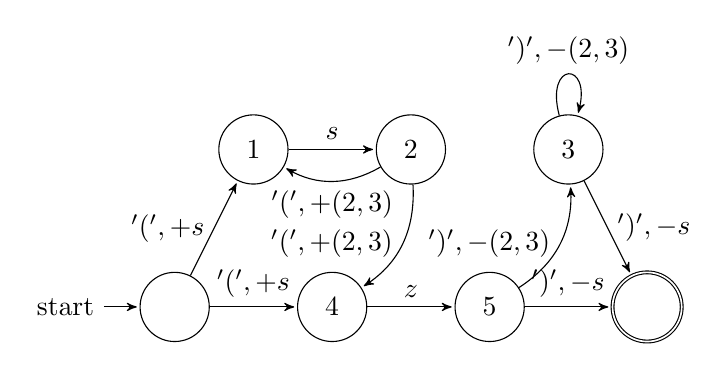
\begin{tikzpicture}[->,>=stealth',shorten >=1pt,auto,node distance=2cm,
    scale = 1,transform shape]

  \node[state] (1) {$1$};
  \node[state] (2) [right of=1] {$2$};
  \node[state] (3) [right of=2] {$3$};
  \node[state] (4) [below of=1, xshift=1cm] {$4$};
  \node[state] (5) [right of=4] {$5$};
  \node[state,initial] (s) [left of=4] {};
  \node[state,accepting] (e) [right of=5] {};

  \draw
  (s) edge[left] node{$'(', +s$} (1)
  (s) edge[above] node{$'(', +s$} (4)
  (3) edge[right] node{$')', -s$} (e)
  (5) edge[above] node{$')', -s$} (e)
  (1) edge[above] node{$s$} (2)
  (4) edge[above] node{$z$} (5)
  (2) edge[bend left, below] node{$'(', +(2, 3)$} (1)
  (2) edge[bend left, left] node{$'(', +(2, 3)$} (4)
  (3) edge[loop above] node{$')', -(2, 3)$} (3)
  (5) edge[left, bend right] node{$')', -(2, 3)$} (3);

\end{tikzpicture}
\end{center}

\noindent The resulting pushdown automaton has only a single source of non-determinism: the edges labelled \verb|'('|. Each one corresponds to one of the allowable child productions at that point in the parse tree.

We now have a pushdown automaton (call it $A_{()}$) that recognizes the top word for each tree in $L(G_t)$. Next we need to be able to add arbitrary parentheses, to produce a word with a rangeset superset. To do this we create a copy of $A_{()}$ with one modification: for every state $s$ in $A_{()}$ (except the initial and final states), add two transitions $s \xrightarrow{'(', +p} s$ and $s \xrightarrow{')', -p} s$. To avoid cluttering the graph too much, these transitions are shown unlabeled below:

\begin{center}
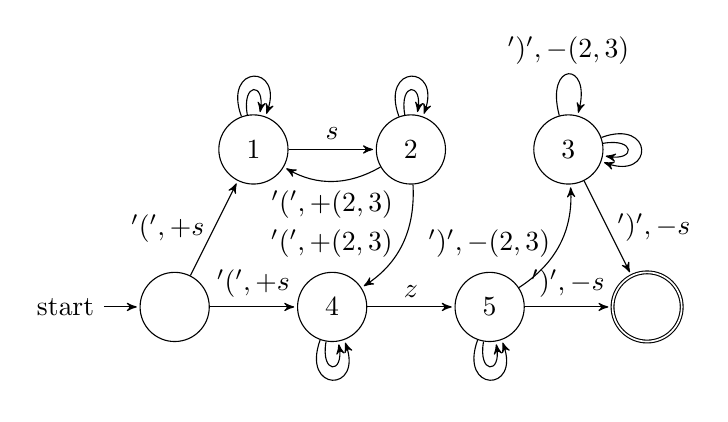
\begin{tikzpicture}[->,>=stealth',shorten >=1pt,auto,node distance=2cm,
    scale = 1,transform shape]

  \node[state] (1) {$1$};
  \node[state] (2) [right of=1] {$2$};
  \node[state] (3) [right of=2] {$3$};
  \node[state] (4) [below of=1, xshift=1cm] {$4$};
  \node[state] (5) [right of=4] {$5$};
  \node[state,initial] (s) [left of=4] {};
  \node[state,accepting] (e) [right of=5] {};

  \draw
  (1) edge[loop, in=80, out=100, looseness=7] node{} (1)
  (1) edge[loop, in=70, out=110, looseness=6] node{} (1)
  (2) edge[loop, in=80, out=100, looseness=7] node{} (2)
  (2) edge[loop, in=70, out=110, looseness=6] node{} (2)
  (3) edge[loop, in=-10, out=10, looseness=7] node{} (3)
  (3) edge[loop, in=-20, out=20, looseness=6] node{} (3)
  (4) edge[loop, in=-80, out=-100, looseness=7] node{} (4)
  (4) edge[loop, in=-70, out=-110, looseness=6] node{} (4)
  (5) edge[loop, in=-80, out=-100, looseness=7] node{} (5)
  (5) edge[loop, in=-70, out=-110, looseness=6] node{} (5)
  (s) edge[left] node{$'(', +s$} (1)
  (s) edge[above] node{$'(', +s$} (4)
  (3) edge[right] node{$')', -s$} (e)
  (5) edge[above] node{$')', -s$} (e)
  (1) edge[above] node{$s$} (2)
  (4) edge[above] node{$z$} (5)
  (2) edge[bend left, below] node{$'(', +(2, 3)$} (1)
  (2) edge[bend left, left] node{$'(', +(2, 3)$} (4)
  (3) edge[loop above] node{$')', -(2, 3)$} (3)
  (5) edge[left, bend right] node{$')', -(2, 3)$} (3);

\end{tikzpicture}
\end{center}

\noindent We will call this automaton $A'_{()}$. Successful runs in this automaton have a surjection to runs in $A_($ (ignore transitions along the newly added edges), and thus also have a surjection to parse trees in $L(G_t)$. We can also note that every sucessful run in $A_{()}$ is also a successful run in $A'_{()}$, since the latter has all states and transitions of the former. Furthermore, two distinct runs, one in $A_{()}$ (call it $p$) and one in $A'_{()}$ (call it $p'$), that both recognize the same word must represent different parse trees in $L(G_t)$. To see why, we consider two cases:

\begin{enumerate}
  \item $p'$ only uses transitions present in $A_{()}$. This is a successful run in $A_{()}$, and distinct from $p$. But there is a bijection between runs in $A_{()}$ and parse trees in $L(T)$, thus $p'$ represents a different parse tree.
  \item $p'$ uses at least one transition added in $A'_{()}$. Using the surjection between runs in $A'_{()}$ and $A_{()}$ we find a new successful run that produces a different word (at least one fewer pair of parentheses). Since this run produces a different word, it must be distinct from $p$, and thus represent a different parse tree.
\end{enumerate}

\noindent Two distinct successful runs that accept the same word thus represent two trees where one permits a superset rangeset of the other. To find such runs we construct a product automaton and trim it. We can construct a product automaton since both $A_{()}$ and $A'_{()}$ are visibly pushdown, with the same partition of the input alphabet (push on open parenthesis, pop on close parenthesis, do nothing otherwise). We can trim the product since it retains the same partitioning and thus is also visibly pushdown.

In this product automaton, if any transition pushes a stack symbol $(a, b)$ where $a \neq b$, or transitions to a state $(p, q)$ where $p \neq q$, then there is a successful run that corresponds to two distinct runs through $A_{()}$ and $A'_{()}$ (since the automaton is trim).

\subsection{Forbidden Children}

\begin{quote}
  \textbf{NOTE:} I had some text here about version 2 of the problem, but I haven't had time to rewrite it to align properly with the lattice formulation, so I've removed it. I'll talk about it during the meeting. Also, I probably need a better title here, this is probably a smidge too dramatic.
\end{quote}

% TODO: this section should be moved to be in the appropriate position {
\newpage

\begin{figure*}[ht]
  \begin{tikzcd}
    L(G_w) & L(G_t) \arrow[l, "\yield"] \\
    L(G'_w) & L(G'_t) \arrow[u, "\semantic"'] \arrow[l, "\yield"]
  \end{tikzcd}
  \caption{The generated grammars and their relation to each other.}
\end{figure*}



\begin{figure*}[ht]
  \begin{subfigure}[b]{.45\linewidth}
    \begin{align*}
      1 + 2 + 3
    \end{align*}
    \caption{Example word in $L(G_w)$.}
  \end{subfigure}
  \begin{subfigure}[b]{.45\linewidth}
      \begin{align*}
        [_S           [_S  &[_N 1 ]_N + \hphantom{[_S} [_N 2 ]_N           ]_S  + [_N 3 ]_N \hphantom{]_S} ]_S \\
        [_S \hphantom{[_S} &[_N 1 ]_N +           [_S  [_N 2 ]_N \hphantom{]_S} + [_N 3 ]_N           ]_S  ]_S
      \end{align*}
    \caption{Example words in $L(G_T)$.}
  \end{subfigure}

  \begin{subfigure}[b]{.45\linewidth}
    \begin{align*}
      1 + 2 + 3
    \end{align*}
    \caption{Example word in $L(G'_w)$.}
  \end{subfigure}
  \begin{subfigure}[b]{.45\linewidth}
      \begin{align*}
        [_S            [_S &[_N 1 ]_N + \hphantom{[_S} [_N 2 ]_N            ]_S + [_N 3 ]_N \hphantom{]_S}]_S \\
        [_S \hphantom{[_S} &[_N 1 ]_N +            [_S [_N 2 ]_N \hphantom{]_S} + [_N 3 ]_N ]_S ]_S
      \end{align*}
    \caption{Example words in $L(G'_T)$.}
  \end{subfigure}
  \caption{Example with an ambiguous word in $L(G'_w)$ with corresponding words from the other grammars.}
  \label{fig:ambig-example-square}
\end{figure*}

\begin{figure*}[ht]
  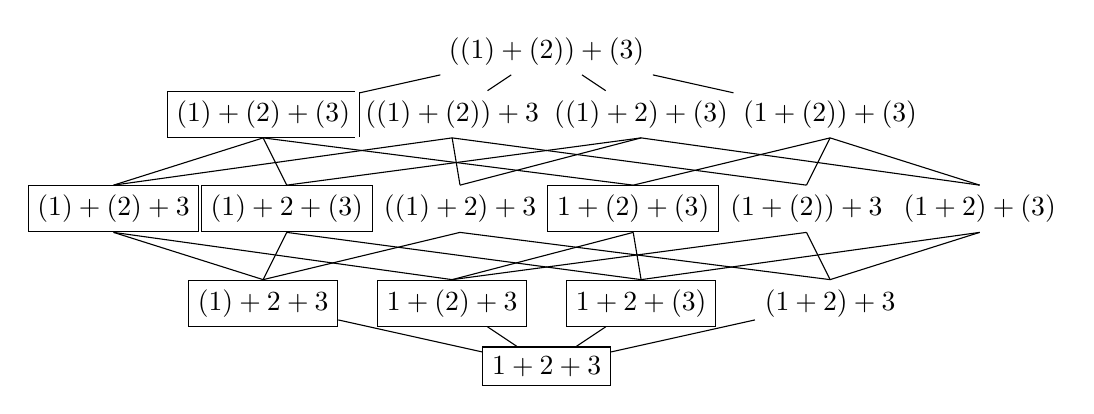
\begin{tikzpicture}[every node/.style={rectangle,draw}]
    \node (a) [draw=white] at (0,5) {$((1) + (2)) + (3)$};

    \node (b1) at (-3.6,4.2) {$(1) + (2) + (3)$};
    \node (b2) [draw=white] at (-1.2,4.2) {$((1) + (2)) + 3$};
    \node (b3) [draw=white] at ( 1.2,4.2) {$((1) + 2) + (3)$};
    \node (b4) [draw=white] at ( 3.6,4.2) {$(1 + (2)) + (3)$};

    \node (c1) at (-5.5,3) {$(1) + (2) + 3$};
    \node (c2) at (-3.3,3) {$(1) + 2 + (3)$};
    \node (c3) [draw=white] at (-1.1,3) {$((1) + 2) + 3$};
    \node (c4) at (1.1,3) {$1 + (2) + (3)$};
    \node (c5) [draw=white] at (3.3,3) {$(1 + (2)) + 3$};
    \node (c6) [draw=white] at (5.5,3) {$(1 + 2) + (3)$};

    \node (d1) at (-3.6,1.8) {$(1) + 2 + 3$};
    \node (d2) at (-1.2,1.8) {$1 + (2) + 3$};
    \node (d3) at ( 1.2,1.8) {$1 + 2 + (3)$};
    \node (d4) [draw=white] at ( 3.6,1.8) {$(1 + 2) + 3$};

    \node (e) at (0, 1) {$1 + 2 + 3$};

  \draw (e) -- (d1);
  \draw (e) -- (d2);
  \draw (e) -- (d3);
  \draw (e) -- (d4);

  \draw (d1.90) -- (c1.270);
  \draw (d1.90) -- (c2.270);
  \draw (d1.90) -- (c3.270);
  \draw (d2.90) -- (c1.270);
  \draw (d2.90) -- (c4.270);
  \draw (d2.90) -- (c5.270);
  \draw (d3.90) -- (c2.270);
  \draw (d3.90) -- (c4.270);
  \draw (d3.90) -- (c6.270);
  \draw (d4.90) -- (c3.270);
  \draw (d4.90) -- (c5.270);
  \draw (d4.90) -- (c6.270);

  \draw (c1.90) -- (b1.270);
  \draw (c1.90) -- (b2.270);
  \draw (c2.90) -- (b1.270);
  \draw (c2.90) -- (b3.270);
  \draw (c3.90) -- (b2.270);
  \draw (c3.90) -- (b3.270);
  \draw (c4.90) -- (b1.270);
  \draw (c4.90) -- (b4.270);
  \draw (c5.90) -- (b2.270);
  \draw (c5.90) -- (b4.270);
  \draw (c6.90) -- (b3.270);
  \draw (c6.90) -- (b4.270);

  \draw (b1) -- (a);
  \draw (b2) -- (a);
  \draw (b3) -- (a);
  \draw (b4) -- (a);
    %%   \draw[preaction={draw=white, -,line width=6pt}] (a) -- (e) -- (c);
  \end{tikzpicture}
  \caption{The lattice of words for the tree $[_S [_S [_N 1 ]_N + [_N 2 ]_N ]_S + [_N 3 ]_N ]_S$ (in $L(G_t)$). The boxed words are shared with Figure~\ref{fig:lattice2}.}
  \label{fig:lattice1}
\end{figure*}


\begin{figure*}[t]

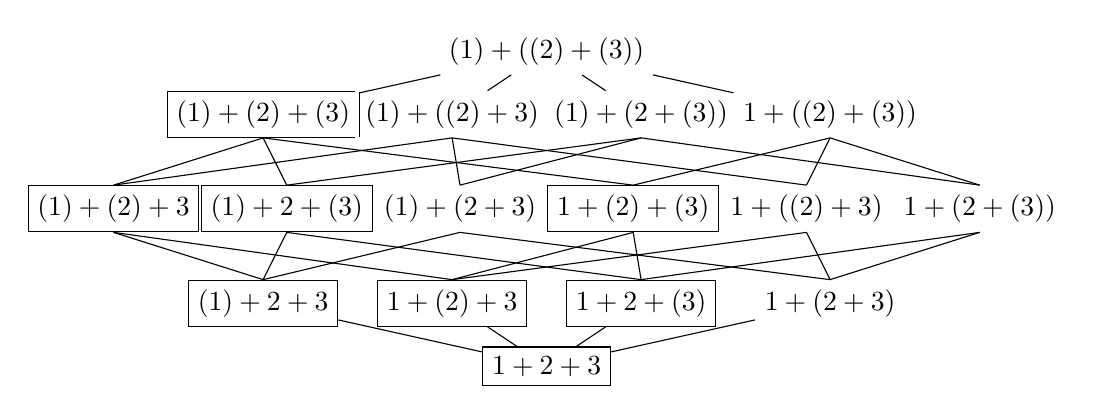
\begin{tikzpicture}[every node/.style={rectangle,draw}]
  \node (a) [draw=white] at (0,5) {$(1) + ((2) + (3))$};

  \node (b1) at (-3.6,4.2) {$(1) + (2) + (3)$};
  \node (b2) [draw=white] at (-1.2,4.2) {$(1) + ((2) + 3)$};
  \node (b3) [draw=white] at ( 1.2,4.2) {$(1) + (2 + (3))$};
  \node (b4) [draw=white] at ( 3.6,4.2) {$1 + ((2) + (3))$};

  \node (c1) at (-5.5,3) {$(1) + (2) + 3$};
  \node (c2) at (-3.3,3) {$(1) + 2 + (3)$};
  \node (c3) [draw=white] at (-1.1,3) {$(1) + (2 + 3)$};
  \node (c4) at (1.1,3) {$1 + (2) + (3)$};
  \node (c5) [draw=white] at (3.3,3) {$1 + ((2) + 3)$};
  \node (c6) [draw=white] at (5.5,3) {$1 + (2 + (3))$};

  \node (d1) at (-3.6,1.8) {$(1) + 2 + 3$};
  \node (d2) at (-1.2,1.8) {$1 + (2) + 3$};
  \node (d3) at ( 1.2,1.8) {$1 + 2 + (3)$};
  \node (d4) [draw=white] at ( 3.6,1.8) {$1 + (2 + 3)$};

  \node (e) at (0, 1) {$1 + 2 + 3$};

  \draw (e) -- (d1);
  \draw (e) -- (d2);
  \draw (e) -- (d3);
  \draw (e) -- (d4);

  \draw (d1.90) -- (c1.270);
  \draw (d1.90) -- (c2.270);
  \draw (d1.90) -- (c3.270);
  \draw (d2.90) -- (c1.270);
  \draw (d2.90) -- (c4.270);
  \draw (d2.90) -- (c5.270);
  \draw (d3.90) -- (c2.270);
  \draw (d3.90) -- (c4.270);
  \draw (d3.90) -- (c6.270);
  \draw (d4.90) -- (c3.270);
  \draw (d4.90) -- (c5.270);
  \draw (d4.90) -- (c6.270);

  \draw (c1.90) -- (b1.270);
  \draw (c1.90) -- (b2.270);
  \draw (c2.90) -- (b1.270);
  \draw (c2.90) -- (b3.270);
  \draw (c3.90) -- (b2.270);
  \draw (c3.90) -- (b3.270);
  \draw (c4.90) -- (b1.270);
  \draw (c4.90) -- (b4.270);
  \draw (c5.90) -- (b2.270);
  \draw (c5.90) -- (b4.270);
  \draw (c6.90) -- (b3.270);
  \draw (c6.90) -- (b4.270);

  \draw (b1) -- (a);
  \draw (b2) -- (a);
  \draw (b3) -- (a);
  \draw (b4) -- (a);
%%   \draw[preaction={draw=white, -,line width=6pt}] (a) -- (e) -- (c);
\end{tikzpicture}
\caption{The lattice of words for the tree $[_S [_N 1 ]_N + [_S [_N 2 ]_N + [_N 3 ]_N ]_S ]_S$ (in $L(G_t)$). The boxed words are shared with Figure~\ref{fig:lattice1}.}
\label{fig:lattice2}
\end{figure*}

\clearpage

% }

\section{Parsetime Ambiguity Reporting} \label{sec:parse-time-reporting}

%% \noindent Generalizing this to a complete grammar, we get the following property: a grammar $G$ is resolvable iff:

%% $$
%% \begin{array}{l}
%%   \forall t \in L(T).\\
%%   \quad \exists w' \in L(G').\\
%%   \qquad \forall t' \in L(T').\ \yield(t') = w' -> \unparen(t') = t
%% \end{array}
%% $$


%%%%%%%%%%%%%%%%%%%%%%%%%%%%%%%%%%%%%%%%%%%%%%%%%%%%%%%%%%%

%% \begin{theorem}
%%   If $\{(, )\} \cap \T = \emptyset$, then any unambiguous word $w \in L(G)$ is resolvable.
%% \end{theorem}

%% \noindent \textbf{Proof.} Since $w$ is unambiguous in $G$ there is exactly one parse tree $t \in L(T)$ such that $\yield(t) = w$. Since $L(G) \subseteq L(G')$ we have that $w \in L(G')$. Furthermore, $w$ is unambiguous in $L(G')$ as well, since no added productions can apply (they all contain parentheses, which cannot be present in $w$). Additionally, since $L(T) \subseteq L(T')$, we have that $t \in L(T')$, and since $\yield(t) = w$, it must be the only parse tree for $w$ in $L(T')$. Finally, $\unparen(t) = t$.

%%%%%%%%%%%%%%%%%%%%%%%%%%%%%%%%%%%%%%%%%%%%%%%%%%%%%%%%%%%

%% %% Acknowledgments
%% \begin{acks}                            %% acks environment is optional
%%                                         %% contents suppressed with 'anonymous'
%%   %% Commands \grantsponsor{<sponsorID>}{<name>}{<url>} and
%%   %% \grantnum[<url>]{<sponsorID>}{<number>} should be used to
%%   %% acknowledge financial support and will be used by metadata
%%   %% extraction tools.
%%   This material is based upon work supported by the
%%   \grantsponsor{GS100000001}{National Science
%%     Foundation}{http://dx.doi.org/10.13039/100000001} under Grant
%%   No.~\grantnum{GS100000001}{nnnnnnn} and Grant
%%   No.~\grantnum{GS100000001}{mmmmmmm}.  Any opinions, findings, and
%%   conclusions or recommendations expressed in this material are those
%%   of the author and do not necessarily reflect the views of the
%%   National Science Foundation.
%% \end{acks}


%% Bibliography
\bibliography{All}


%% %% Appendix
%% \appendix
%% \section{Appendix}

%% Text of appendix \ldots

\end{document}
